\documentclass[12pt,a4paper]{book}
\usepackage[utf8]{inputenc}
\usepackage[pdftex]{graphicx}
\usepackage[italian]{babel}
\usepackage{fixltx2e,bold-extra,geometry,
    amssymb,amsmath,mathtools, microtype,url,cite}
\usepackage[bookmarks=true, hidelinks, pdftitle={
RELAZIONE FINALE ATTIVITA' PROGETTUALE DI SISTEMI DIGITALI M},
pdfauthor={Gabriele Tornatore}]{hyperref}
% \pagestyle{headings}
\graphicspath{{images/}}

\usepackage{float} %use H in pictures

\usepackage{hyperref} % link color
\hypersetup{
    colorlinks=true,
    linkcolor=black,   
    urlcolor=blue,
}

\usepackage{pgfplots} % graphics

%%%%%%%%%%%%%%%%% Python Code %%%%%%%%%%%%%%%%%%%%%%%%%%%%%%%%%%%%%%%%%%%%%%%%%

% Default fixed font does not support bold face
\DeclareFixedFont{\ttb}{T1}{txtt}{bx}{n}{8} % for bold
\DeclareFixedFont{\ttm}{T1}{txtt}{m}{n}{8} % for normal

% Custom colors
\usepackage{color}
\definecolor{deepblue}{rgb}{0.45,0.95,0.36}
\definecolor{deepred}{rgb}{0,0,0}
\definecolor{deepgreen}{rgb}{0.67,0.31,0.31}
\definecolor{deepblack}{rgb}{0.11,0.11,0.11}
\definecolor{lightblue}{rgb}{0.77, 0.89, 0.93}
\definecolor{codeblack}{rgb}{0.20,0.20,0.20}
\definecolor{codered}{rgb}{1,0.6,0.6}
\definecolor{codelightblue}{rgb}{0.6,0.6,0.6}
\definecolor{codegray}{rgb}{0.5,0.5,0.5}


\usepackage{listings}

% Python style for highlighting
\newcommand\pythonstyle{\lstset{
	backgroundcolor=\color{codeblack},
	language=Python,
	basicstyle=\fontsize{8}{8}\ttm\color{white},
	morekeywords={self},
	keywordstyle=\fontsize{8}{8}\ttb\color{deepblue},
	emph={MyClass,__init__},
	emphstyle=\fontsize{8}{8}\ttb\color{codered},
	stringstyle=\fontsize{8}{8}\ttm\color{deepgreen},
	commentstyle=\fontsize{8}{8}\ttm\color{codelightblue},
	breaklines=true,
	frameround=ftff,
	frame=single,
	showstringspaces=false,
	numbers=left,
	numberstyle=\ttm\color{codegray},
	stepnumber=1,
	numbersep=8pt,
    belowcaptionskip=5em,
    belowskip=3em
}}

\makeatletter
\lst@CCPutMacro
    \lst@ProcessOther {"2D}{\lst@ttfamily{-{}}{-}}
    \@empty\z@\@empty
\makeatother

\makeatletter
\lst@CCPutMacro
    \lst@ProcessOther {"3C}{\lst@ttfamily{<{}}{<}}
    \@empty\z@\@empty
\makeatother

\makeatletter
\lst@CCPutMacro
    \lst@ProcessOther {"3E}{\lst@ttfamily{>{}}{>}}
    \@empty\z@\@empty
\makeatother

% Python environment
\lstnewenvironment{python}[1][]
{
	\pythonstyle
	\lstset{#1}
}
{}

% Python for external files
\newcommand\pythonexternal[2][]{{
		\pythonstyle
		\lstinputlisting[#1]{#2}}}

% Python for inline
\newcommand\pythoninline[1]{{\pythonstyle\lstinline!#1!}}

%%%%%%%%%%%%%%%%% Normal Text Code %%%%%%%%%%%%%%%%%%%%%%%%%%%%%%%%%%%%%%%%%%%%%%%%%

% normal text style for highlighting
\newcommand\textnormalstyle{\lstset{
		backgroundcolor=\color{codeblack},
		basicstyle=\fontsize{8}{8}\ttm\color{white},
		keywordstyle=\fontsize{8}{8}\ttm\color{white},
		emphstyle=\fontsize{8}{8}\ttm\color{white},    % Custom highlighting style
		stringstyle=\fontsize{8}{8}\ttm\color{white},
		commentstyle=\fontsize{8}{8}\ttm\color{white},
		breaklines=true,
		showstringspaces=false
}}

% txt for external files
\newcommand\textexternal[2][]{{
		\textnormalstyle
		\lstinputlisting[#1]{#2}}}
		
%%%%%%%%%%%%%%%%% Swift Code %%%%%%%%%%%%%%%%%%%%%%%%%%%%%%%%%%%%%%%%%%%%%%%%%

\lstdefinelanguage{swift}
{
  keywords=[1]{UInt8, Float32, Bool, Bundle, UIViewController, MemoryLayout, Data, UnsafeMutableBufferPointer},
  keywords=[2]{
    open,catch,@escaping,nil,throws,func,if,then,else,for,in,while,do,switch,case,default,where,break,continue,fallthrough,return,
    typealias,struct,class,enum,protocol,var,func,let,get,set,willSet,didSet,inout,init,deinit,extension,
    subscript,prefix,operator,infix,postfix,precedence,associativity,left,right,none,convenience,dynamic,
    final,lazy,mutating,nonmutating,optional,override,required,static,unowned,safe,weak,internal,
    private,public,is,as,self,unsafe,dynamicType,true,false,nil,Type,Protocol,try,guard
  },
  keywords=[3]{copy, invoke, allocateTensors, data},
  keywords=[4]{main,path,memcpy,append,allocate,size,copyBytes},
  keywords=[5]{loadModel},
  keywords=[6]{Interpreter,TfliteModel},
  morecomment=[l]{//}, % l is for line comment
  morecomment=[s]{/*}{*/}, % s is for start and end delimiter
  morestring=[b]", % defines that strings are enclosed in double quotes
}

\definecolor{lightblue}{rgb}{0.24,0.46,0.53}
\definecolor{lightgreen}{rgb}{0.40,0.63,0.59}
\definecolor{lightgreen2}{rgb}{0.51,0.71,0.67}
\definecolor{pink}{rgb}{0.86,0.43,0.62}
\definecolor{lightpurple}{rgb}{0.70,0.60,0.82}
\definecolor{purple}{rgb}{0.53,0.41,0.71}
\definecolor{string}{rgb}{0.92,0.47,0.42}
\definecolor{comment}{rgb}{0.44,0.48,0.52}

\newcommand\swiftstyle{\lstset{
  backgroundcolor=\color{codeblack},
  language=swift,
  extendedchars=true,
  basicstyle=\fontsize{8}{8}\ttm\color{white},
  keywordstyle=[1]\fontsize{8}{8}\ttb\color{lightpurple},
  keywordstyle=[2]\fontsize{8}{8}\ttb\color{pink},
  keywordstyle=[3]\fontsize{8}{8}\ttb\color{lightgreen},
  keywordstyle=[4]\fontsize{8}{8}\ttb\color{purple},
  keywordstyle=[5]\fontsize{8}{8}\ttb\color{lightblue},
  keywordstyle=[6]\fontsize{8}{8}\ttb\color{lightgreen2},
  stringstyle=\fontsize{8}{8}\ttm\color{string},
  commentstyle=\fontsize{8}{8}\ttm\color{comment},
  breaklines=true,
  frameround=ftff,
  frame=single,
  showspaces=false,
  showstringspaces=false,
  numbers=left,
  numberstyle=\ttm\color{codegray},
  numbersep=9pt,
  tabsize=3,
  showtabs=false,
  belowskip=3em
}}

% swift for external files
\newcommand\swiftexternal[2][]{{
		\swiftstyle
		\lstinputlisting[#1]{#2}}}

%%%%%%%%%%%%%%%%% New Commands %%%%%%%%%%%%%%%%%%%%%%%%%%%%%%%%%%%%%%%%%%%%%%%%%
%
\newcommand{\intentblankpage}{
%     Leaves a blank page
    \newpage
    \null
    \vfill
    \thispagestyle{empty}
    \begin{center}
%         \textit{This page intentionally left blank.}
        \textit{Questa pagina \`e lasciata intenzionalmente bianca.}
    \end{center}
    \newpage
}
% 
% Writes intentionally blank page when there is a \newpage on the left page of
% a book.
\makeatletter
    \def\cleardoublepage{\clearpage%
        \if@twoside
            \ifodd\c@page\else
                \vspace*{\fill}
                \hfill
                \begin{center}
%                     \textit{This page intentionally left blank.}
                    \textit{}
                \end{center}
                \thispagestyle{empty}
                \newpage
                \if@twocolumn\hbox{}\newpage\fi
            \fi
        \fi
    }
\makeatother
%
% Length to set margins for 65 chars
\newlength{\sixtyfivecharwidth}
\settowidth{\sixtyfivecharwidth}{
    \normalfont abcdefghijklmnopqrstuvwxyzabcdefghijklmnopqrstuvwxyz1234567890123}
% 
%Integral with the limit below(mathrlap)
% \newcommand{\intlimr}[1]{\ensuremath{\int \limits_{\mathrlap{#1}}}}
% 
% This redefine could cause big issues! See: 
% http://tex.stackexchange.com/questions/248421/use-mathclap-as-default-in-limits-of-integration
% \let\oldlimits\limits
% \def\limits_#1{\oldlimits_{\mathclap{#1}}}
\def\mclimits_#1{\limits_{\mathclap{#1}}}
%%%%%%%%%%%%%%%% End New Commands %%%%%%%%%%%%

\begin{document}
    \pagenumbering{Roman}
    % \newgeometry{margin=26mm} % allarga la pagina anche in altezza
\newgeometry{lmargin=26mm,rmargin=26mm}
\begin{titlepage}
\begin{center}
    {{\Large{\textsc{Alma Mater Studiorum $\cdot$ Universit\`a di
    Bologna}}}}
	\rule[0.1cm]{15.8cm}{0.1mm}
    \rule[0.5cm]{15.8cm}{0.6mm}
    {\normalsize{\textsc { Scuola di Ingegneria e Architettura\\
    \vspace{5mm}
    Dipartimento di Informatica - Scienza e Ingegneria -\\
    \vspace{5mm}
    Corso di Laurea Magistrale in Ingegneria Informatica}}}\\
	\vspace{10mm}
	{\small{\sc Anno Accademico 2021/2022}}%inserire l'anno accademico a cui si è iscritti
\end{center}
\vspace{10mm}
\begin{center}
    {\LARGE\textbf{- RELAZIONE FINALE -}}\\
    \vspace{3mm}
    {\LARGE\textbf{RICONOSCIMENTO}}\\
    \vspace{3mm}
    {\LARGE\textbf{DI GENERI MUSICALI}}\\
    \vspace{3mm}
    {\LARGE{\bf TRAMITE L'USO DI CNN}}\\
    \vspace{10mm} {\large{\sc Corso di Attività Progettuale di Sistemi Digitali M}}
\end{center}
\vfill
\par
\noindent
\begin{minipage}[t]{0.47\textwidth}
    {\large{\sc Autore:}\\
    {\bf \textsc{Gabriele Tornatore}}}\\
\end{minipage}
\vspace{20mm}
\end{titlepage}
\restoregeometry

    
    \tableofcontents
    
    \chapter*{Introduzione} \pagenumbering{arabic}
    \addcontentsline{toc}{chapter}{Introduzione}
    \label{CH:Intro}
    La musica ha assunto un ruolo di primo piano nella storia dell'uomo. Forse è la voglia di esprimere i propri sentimenti e le proprie emozioni che hanno obbligato l'essere umano a comporre sempre nuovi brani. Senza alcun dubbio, la chitarra è uno degli strumenti più usati. Per esempio, quando si va in campeggio e alla sera ci si siede davanti al falò, sono proprio le sue note a riempire l'aria.\\ Il tema libero lasciato dai professori ha permesso di approfondire ma soprattutto conoscere meglio il vastissimo campo della musica.  \\ Il progetto ha l'obiettivo di trascrivere in modo automatico le tablature per chitarra tramite l'utilizzo di reti neurali convoluzionali (\textit{CNN}) in modo che anche chi non è in grado di suonare questo strumento lo possa fare. Il tutto funziona tramite l'ausilio di un semplice \textit{smartphone}. \\

La relazione è articolata come segue:
\begin{itemize}
	\item nel \textbf{capitolo 1} viene descritta brevemente la chitarra;
	\item nel \textbf{capitolo 2} viene introdotto il dominio in cui lavoreremo;
	\item nel \textbf{capitolo 3} viene descritto il modello della nostra rete, l'addestramento che è stato eseguito e la sua accuratezza;
	\item nel \textbf{capitolo 4} viene realizzata l'implementazione sul dispositivo \textit{embedded}, nel nostro caso sono gli \textit{smartphone};
	\item il \textbf{capitolo 5} conclude la relazione presentando i risultati ottenuti, gli obiettivi raggiunti ed eventuali problematiche che potrebbero essere risolte in futuro.
\end{itemize}
La relazione è stata scritta come un \textit{diario} mettendo in risalto tutti i passaggi, i tentativi e i problemi che si sono verificati.\\
\newline
Il codice, il modello e i \textit{log} di tutto il progetto possono essere reperiti nella seguente repository git: \href{https://github.com/it9tst/tab-writer}{https://github.com/it9tst/tab-writer} 
 
    
    \chapter{Set dati utilizzati}
    \label{CH:Teoria}
    La chitarra ha una lunga tradizione che affonda le sue radici addirittura al tempo degli arabi. I primi esemplari risalgono al tredicesimo secolo. Inizialmente dotata di quattro corde, si è accresciuta nel Rinascimento di un'altra corda, arrivando poi nel periodo Barocco all'attuale numero di sei.\\
\newline
La chitarra è composta da due parti principali:
\begin{itemize}
	\item il \textbf{manico}, su cui si trova la tastiera e che termina con la paletta la quale ospita le meccaniche per l'accordatura;
	\item la \textbf{cassa di risonanza} o tavola armonica con una cavità centrale, che serve ad amplificare il suono prodotto dalle corde.
\end{itemize}

\begin{figure}[H]
	\centering
	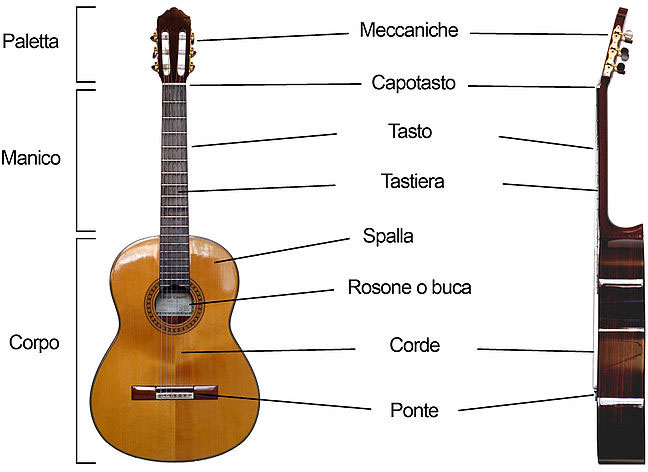
\includegraphics[scale=0.50]{./images/img14.jpg}
\end{figure}

\subsection{Corde}
Le corde delle chitarre moderne sono sei e sono ordinate dall'alto verso il basso nel seguente modo:
\begin{itemize}
	\item la prima corda corrisponde alla nota \textit{Mi cantino} (e);
	\item la seconda corrisponde alla nota \textit{Si} (B);
	\item la terza corrisponde alla nota \textit{Sol} (G);
	\item la quarta corrisponde alla nota \textit{Re} (D);
	\item la quinta corrisponde alla nota \textit{La} (A);
	\item la sesta corrisponde alla nota \textit{Mi basso} (E).
\end{itemize}
L'ultima corda dell'elenco è quella più spessa, mentre la prima è la più sottile.

\begin{figure}[H]
	\centering
	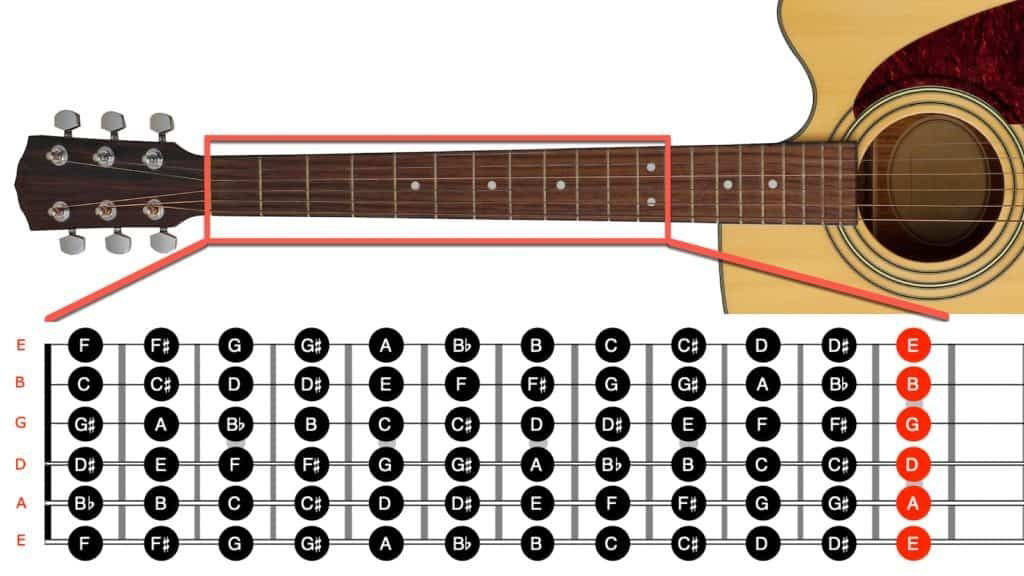
\includegraphics[scale=0.35]{./images/img12.jpg}
\end{figure}

\subsection{Tasti}
Sul manico della chitarra c’è la tastiera. Si chiama tastiera proprio perchè ci sono i tasti. Quest'ultimi sono delimitati da delle barrette di metallo e ognuno di essi corrisponde a una nota. Dunque, se abbiamo una chitarra a diciannove tasti, possiamo fare diciannove note diverse per ogni corda.\\
La distanza tra due tasti della stessa corda prende il nome di \textbf{semitono}. Ad esempio, se premiamo la sesta corda in corrispondenza del \textit{La}, poi premendo la corda al tasto adiacente più vicino alla cassa di risonanza (un semitono più alto) ascolteremo un \textit{La\#}. Se non premiamo nessun tasto la corda si dice che è suonata a vuoto. Le sei corde suonate a vuoto devono emettere dei suoni ben precisi. Dunque, la chitarra deve essere accordata. L'accordatura classica delle sei corde, ovvero la nota che devono suonare le corde a vuoto (dal basso all'alto), è la seguente: \textit{Mi}, \textit{La}, \textit{Re}, \textit{Sol}, \textit{Si}, \textit{Mi}. \\ Conoscendo il suono prodotto dalle sei corde suonate a vuoto e sapendo che ogni nota suonata ad un tasto dista di un semitono dalla nota suonata al tasto adiacente possiamo mappare tutta la tastiera della chitarra.
\begin{figure}[H]
	\centering
	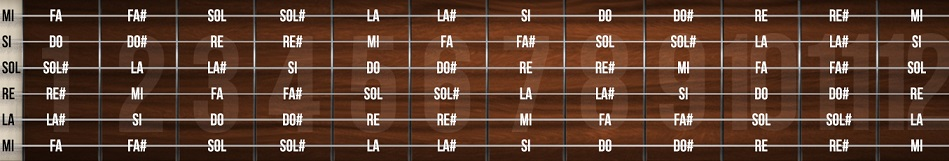
\includegraphics[scale=0.60]{./images/img13.jpg}
\end{figure}

\subsection{Tab}
La \textit{tab} è una rappresentazione delle corde della chitarra. Una tablatura è solitamente scritta usando sei linee orizzontali, ognuna corrispondente a una corda.\\
Al contrario dei normali spartiti, su una tablatura non ci sono le note da suonare ma si trovano le indicazioni su dove mettere le dita.\\I numeri sulle linee corrispondono ai tasti della tastiera. Ad esempio, un "1" sulla prima corda, indica di suonare il \textit{Mi cantino}, tenendo premuto il primo tasto.\\
Se il numero è maggiore o uguale a uno, bisogna premere il tasto corrispondente quando si suonerà quella corda. Se troviamo uno \textbf{zero} allora si suona la corda a vuoto, senza premere alcun tasto.
\begin{figure}[H]
	\centering
	\includegraphics[scale=0.55]{./images/img15.png}
\end{figure}
\noindent Spesso leggendo una tablatura si trovano dei numeri che sono allineati verticalmente. In questo caso si premono più tasti contemporaneamente. Le \textit{tab} vanno lette come libri cioè da sinistra a destra.
\begin{figure}[H]
	\centering
	\includegraphics[scale=0.55]{./images/img16.png}
\end{figure}
    
    \chapter{Architettura e addestramento del modello}
    \label{CH:Val_num}
    Le note musicali si possono classificare nel seguente modo:
\begin{figure}[H]
	\centering
	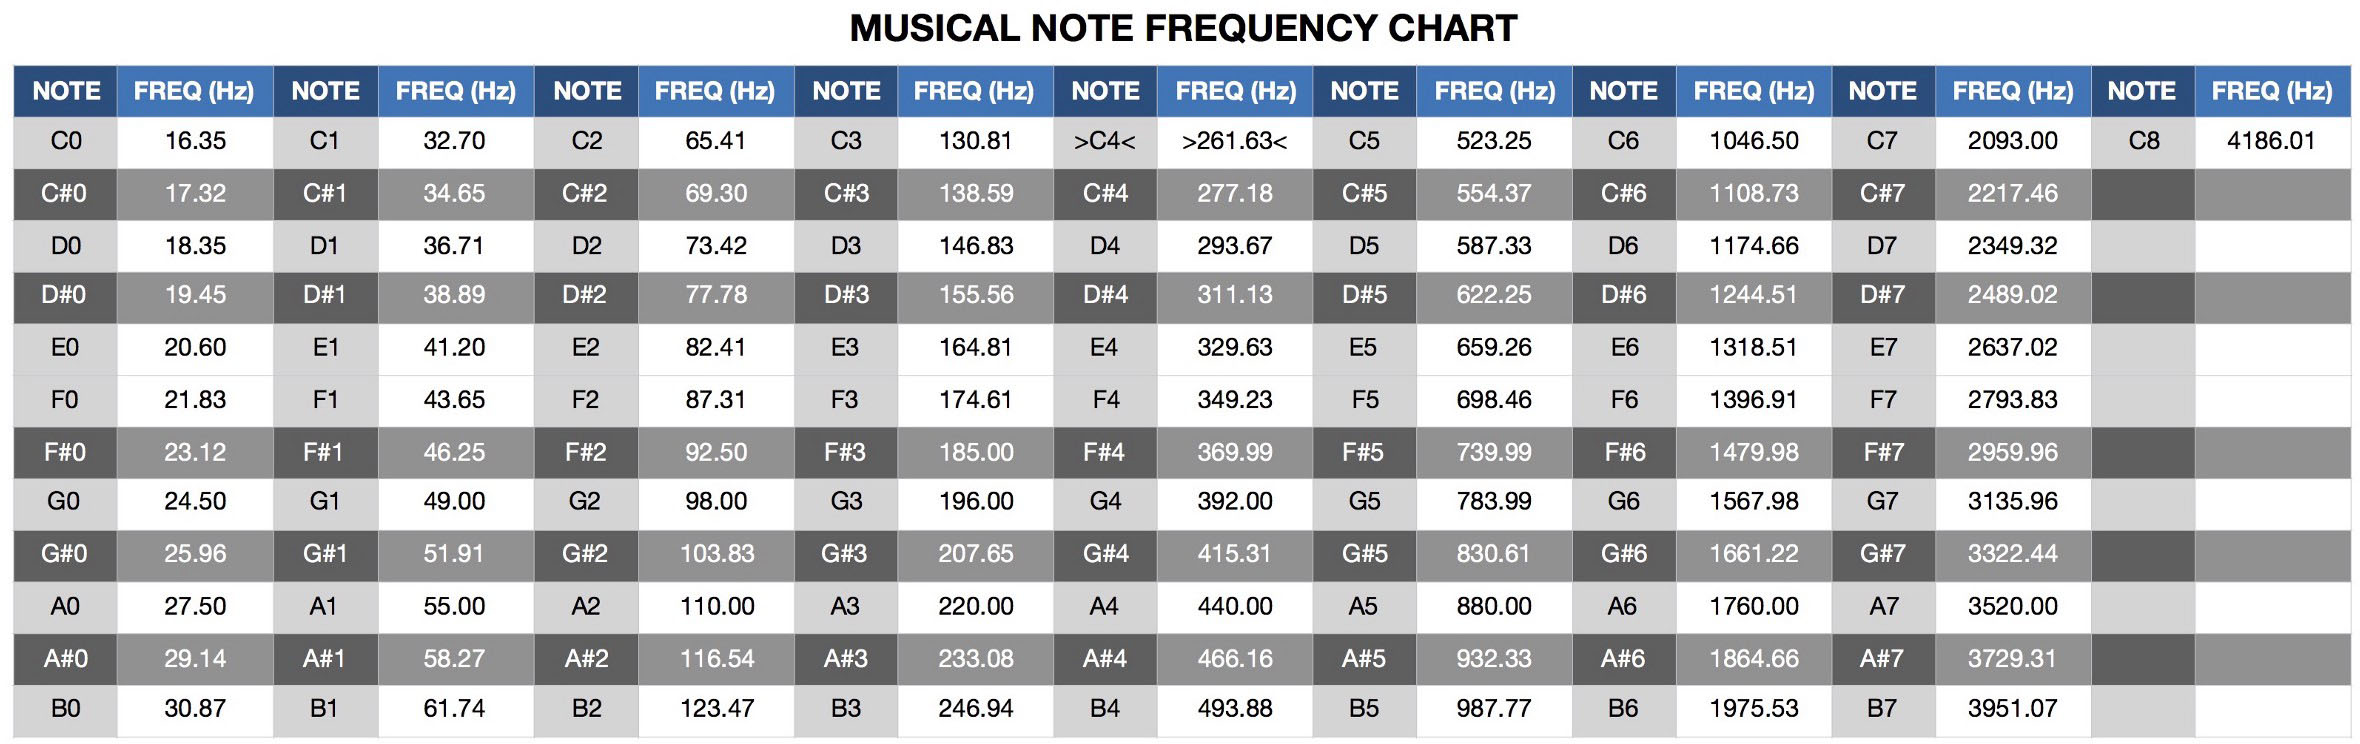
\includegraphics[scale=0.17]{./images/img4.jpg}
\end{figure}
\noindent La lettera a sinistra identifica la nota musicale mentre il numero a destra rappresenta la sua frequenza.\\
In musica, un'\textbf{ottava} è l'intervallo di otto note posizionate a frequenza diversa nella scala musicale. Le frequenze intermedie sono altre sei note. La frequenza tra una nota di un'ottava e la stessa nota di un'ottava successiva è doppia. Per esempio, il \textit{La} centrale (A4) ha frequenza di 440 Hz, il \textit{La} (A5) posto un'ottava sopra ha frequenza 880 Hz, quello un'ottava sotto (A3) ha frequenza 220 Hz.\\
Se si rappresentassero le prime sei ottave della nota \textit{Do} (C) potremmo vedere che la sua frequenza raddoppia ad ogni ottava.\\
\newline
I tasti che intercorrono fra gli estremi della stessa ottava (esempio \textit{Do} (C4) - \textit{Do} (C5)) sono dodici semitoni per cui la frequenza deve raddoppiare ogni dodici semitoni. Si può rappresentare quanto detto dalla seguente formula:
\vspace*{2ex}
\begin{center}
	\begin{math}
		F_{k}=440Hz \cdot 2^{k \over 12}
	\end{math}
\end{center}

Nel campo della musica viene utilizzata la trasformata a Q costante, a discapito della più nota trasformata di Fourier, proprio per la sua natura esponenziale. Inoltre, l'accuratezza della trasformata a Q costante è analoga alla scala logaritmica e imita l'orecchio umano, avendo una risoluzione di frequenza più alta a quelle più basse e una risoluzione più bassa alle frequenze più alte. Infatti, dal seguente grafico si può notare la natura esponenziale della funzione:
\vspace*{2ex}
\begin{center}
	\begin{tikzpicture}
	\begin{axis}[ 
		xlabel=$k$,
		ylabel={$frequenza$}
		] 
		\addplot {440*2^x/12}; 
	\end{axis}
\end{tikzpicture}
\end{center}
    
    \chapter{Implementazione su dispositivo Embedded}
    \label{CH:Val_num}
    Per dispositivo \textit{embedded} si intende un dispositivo piccolo e compatto con consumi energetici molto contenuti. Proprio per queste caratteristiche sono usati per il \textit{deployment} di reti neurali.

\section{Conversione del modello da Keras a Tensorflow Lite}
Il modello è stato convertito in \textit{Tensorflow Lite}. Il seguente codice consente di caricare il modello addestrato tramite \textit{Tensorflow} e di convertirlo nel formato .\textit{tflite} pronto per essere utilizzato su un dispositivo \textit{embedded}.\\
\newline Il convertitore ha il compito di ottimizzare il modello riducendo le sue dimensioni e aumentando la sua velocità di esecuzione.
\vspace*{2ex}
\pythonexternal{./codes/tensorflowLite.py}
\noindent Il Jupyter notebook dove si trova il codice anche per gli altri modelli dell'albero si trova nel file \textit{"5 - Model tflite.ipynb"}.

\section{Sviluppo applicazione Android}
\subsection{Sviluppo applicazione con Java 1.8 e Android Studio 4.1.2}
L'applicazione è stata creata in \textit{Java} con \textit{Android Studio}, che è un ambiente di sviluppo integrato per lo sviluppo per la piattaforma \textit{Android}.
\begin{figure}[H]
	\centering
	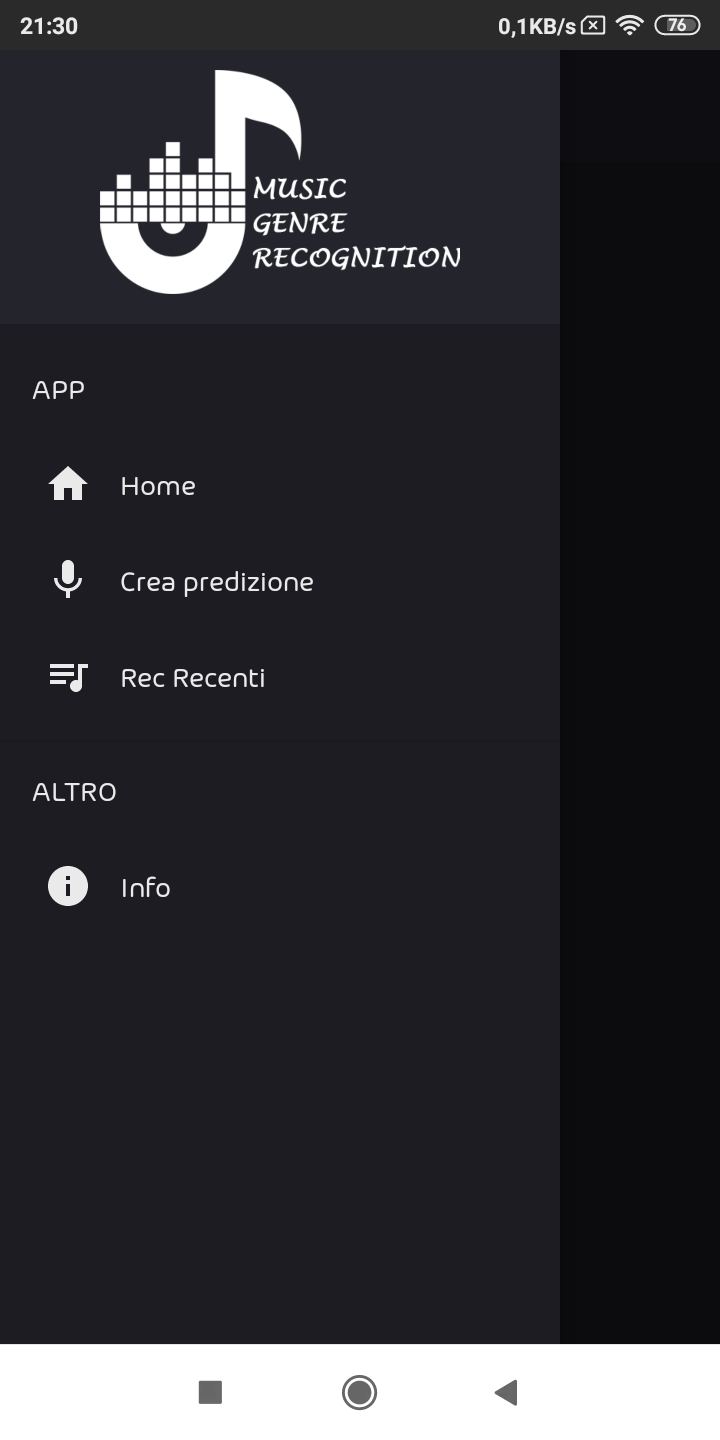
\includegraphics[scale=0.20]{./images/mobile01.jpg}
	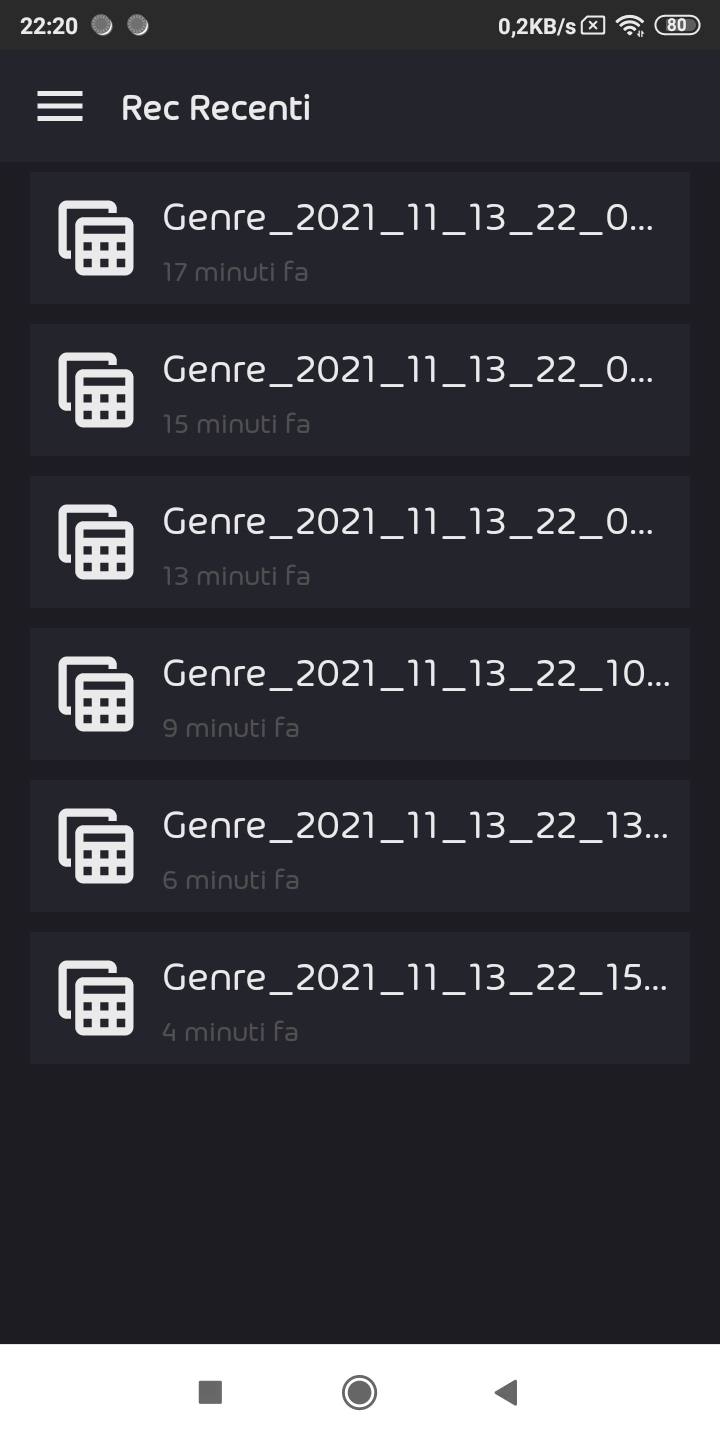
\includegraphics[scale=0.20]{./images/mobile02.jpg}
\end{figure}
\noindent Sono state create un paio di interfacce con elementi grafici ed è stato implementato un \textit{database} che tiene traccia del risultato delle registrazioni predette, in modo da poterle consultare anche in un secondo momento senza dover richiamare l'interprete di \textit{Tensorflow Lite}.\\
\newline
Per avviare la registrazione, basta cliccare sul pulsante centrale su cui è raffigurato un microfono. A questo punto il cellulare registra l'audio e per terminarla bisogna ricliccare sul pulsante.
\begin{figure}[H]
	\centering
	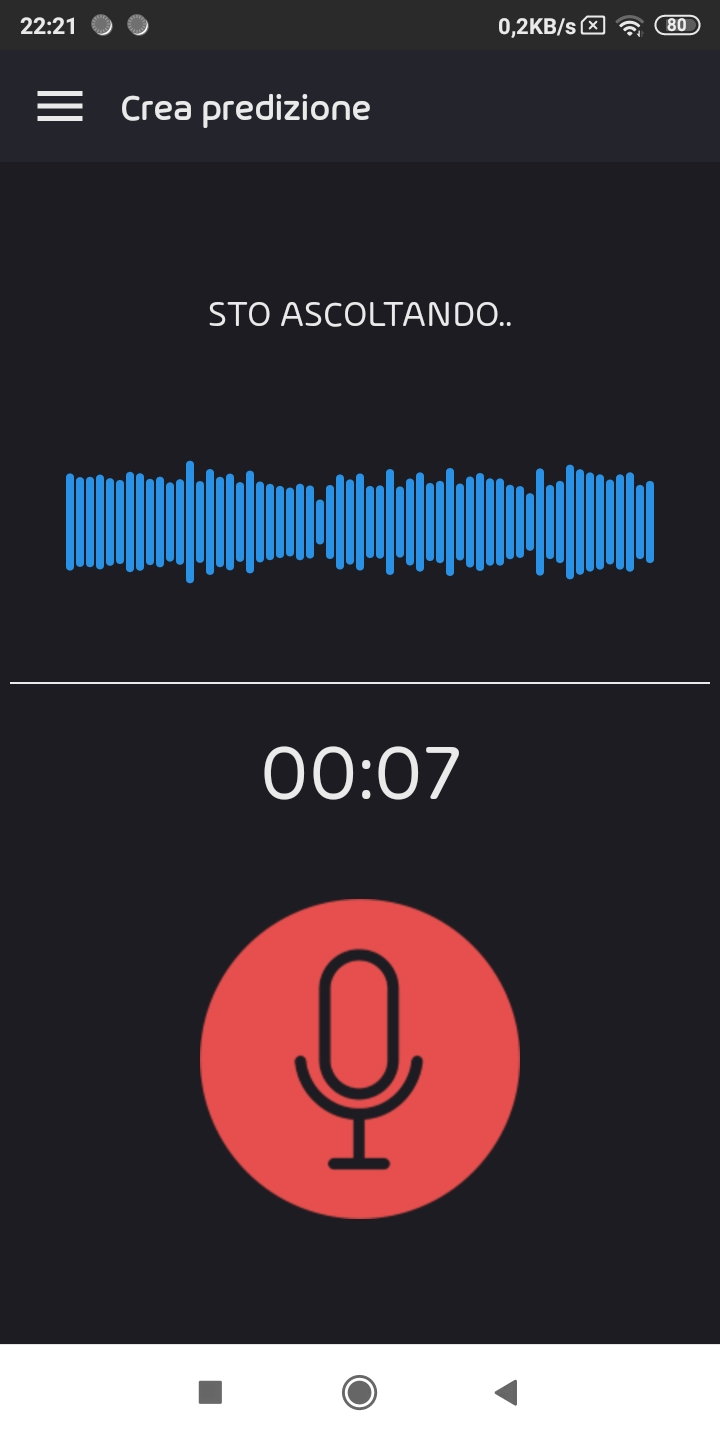
\includegraphics[scale=0.20]{./images/mobile03.jpg}
	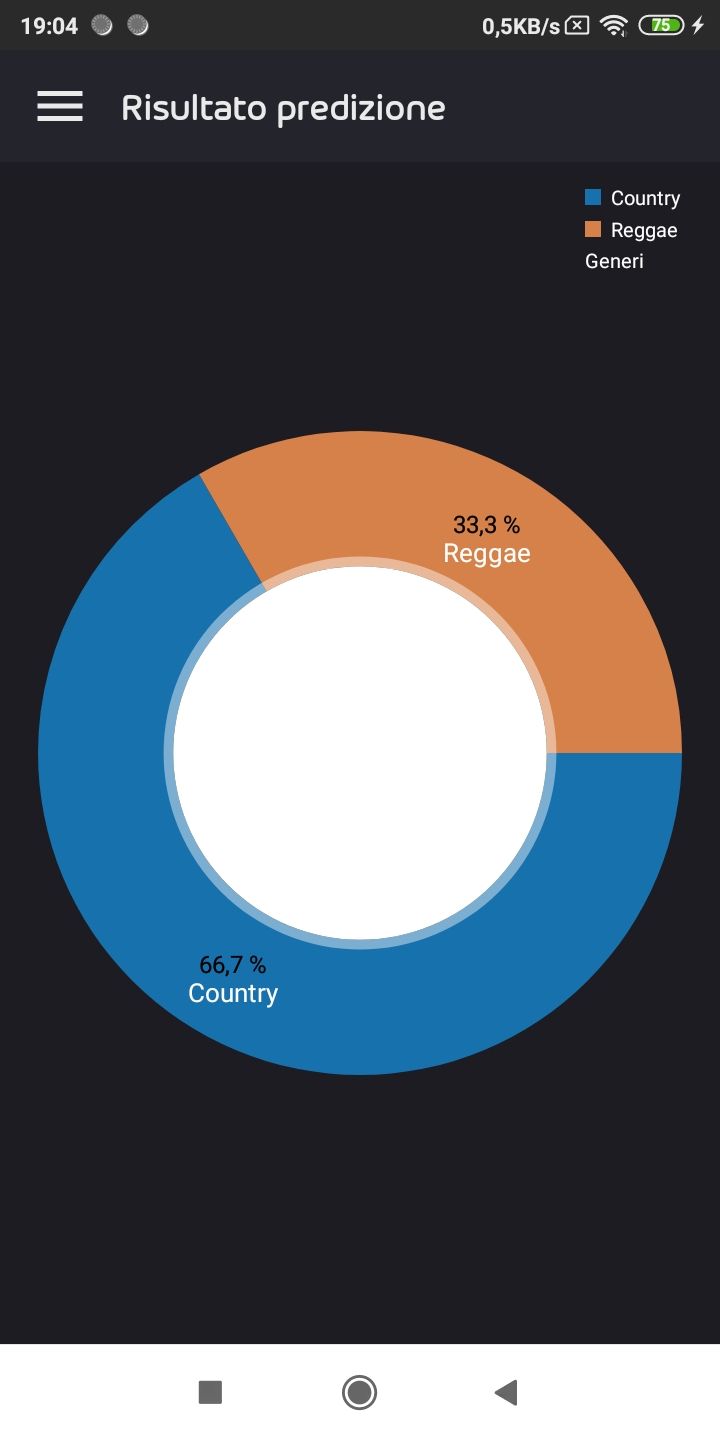
\includegraphics[scale=0.20]{./images/mobile04.jpg}
\end{figure}
\noindent A questo punto il file verrà salvato sul cellulare e convertito nel formato .\textit{wav}. Una volta aver ricavato le immagini dal \textit{file} audio, grazie al modello della rete è possibile avviare la predizione. Dopodiché il risultato apparirà in una nuova interfaccia.\\
\newline Per ricavare lo spettrogramma dalle registrazioni audio e per gestire la predizione è stato usato \textit{chaquopy}, un \textit{plugin} che consente di implementare codice \textit{Python} all'interno delle applicazioni \textit{Android}.

\subsection{Implementazione di Tensorflow Lite}
Una volta ottenuti gli \textit{input} della rete, possiamo eseguire l'inferenza con il modello.\\ Per predire correttamente il modello con l'albero decisionale è stato necessario creare una classe \textit{ModelNodeTree} che, essendo dinamica, funzioni con qualsiasi tipo e grandezza di albero.\\
Una volta passato il path del modello, relativo al nodo da predire, rendiamo accessibile l'interprete di \textit{Tensorflow Lite}, allochiamo i tensori ed estrapoliamo dal modello rispettivamente il tipo e il formato dell'\textit{input} e dell'\textit{output}. Passiamo il batch da predire tramite la funzione \textit{interpreter.set\_tensor()}, invochiamo l'interprete e tramite la funzione \textit{interpreter.get\_tensor()} otteniamo una copia dei valori provenienti dal tensore di \textit{output}.\\
In base al risultato, continuiamo la discesa dell'albero verso il ramo destro o sinistro, ricorsivamente, fino al nodo radice.
\vspace*{2ex}
\pythonexternal{./codes/mobile01.py}
\noindent Infine, i risultati vengono salvati in un \textit{JSON} e conservati nel \textit{database} dell'applicazione.
\vspace*{2ex}
\pythonexternal{./codes/mobile02.py}
    
    \chapter{Conclusioni}
    \label{CH:Concl}
    Sulle due applicazioni sono stati eseguiti diversi \textit{test} e possiamo affermare che si comportano entrambe abbastanza bene. Certamente, il progetto potrebbe essere migliorato perchè i limiti individuati sono i seguenti:
\begin{itemize}
		\item Se si suonassero ad esempio, le note 64 e 65 della prima corda in sequenza, la rete potrebbe predire una delle due note, o tutte e due, non sulla stessa corda ma in quella successiva. Questo non sarebbe un errore perchè il suono è lo stesso ma in certi casi sarebbe meglio suonare tasti vicini per una questione di manualità. Ciò accade perchè il sistema determina la tablatura finestra per finestra e non tiene conto della sequenza della registrazione;
		\item Se la canzone è troppo veloce, cioè ha un tempo o BPM (battiti per minuto) alto, la predizione tende ad essere errata;
		\item Alcune note potrebbero non essere riconosciute perchè c'è ancora un margine di errore di quasi il 10\%.
	\end{itemize}
Nonostante tutto, siamo molto soddisfatti del progetto che è stato realizzato. Grazie a questa materia abbiamo esplorato due mondi che per noi erano sconosciuti come lo sviluppo di applicazioni \textit{mobile}. Siamo consapevoli che abbiamo perlustrato solo una piccola parte di questa vastissima materia ma quello che abbiamo appreso sarà sicuramente usato come base di partenza per progetti futuri.\\
\newline
A fini dimostrativi, forniamo insieme alla documentazione un breve video dell'applicazione in funzione.
    
%     \nocite{*}
    \bibliographystyle{IEEEtran}
    %%%%%%%%%%% Example 1%%%%%%%%%%%%%%%%%%%%%%%%%%
    \begin{thebibliography}{100}  % 100 is a random guess of the total number of %references
    
    \bibitem{HK} \textit{Genere musicale}. (s.d.). Wikipedia, l'enciclopedia libera. Ultimo accesso: 11 novembre 2021, https://it.wikipedia.org/wiki/Genere\_musicale
    
    \bibitem{HK} \textit{Generi musicali, teorie e criteri di classificazione}. (s.d.). Note tra le righe. Ultimo accesso: 11 novembre 2021, https://www.notetralerighe.it/teoria-musicale/generi-musicali
    
    \bibitem{HK} \textit{Learning to Recognize Musical Genre from Audio}. (s.d.). Papers With Code. Ultimo accesso: 11 novembre 2021, https://paperswithcode.com/paper/learning-to-recognize-musical-genre-from
    
    \bibitem{HK} \textit{Tecniche di ottimizzazione II}. (s.d.). Aaron Defazio. https://atcold.github.io/pytorch-Deep-Learning/it/week05/05-2/
    
    \bibitem{HK} \textit{Comprendere la discesa del gradiente e l'ottimizzazione di Adam}. (s.d.). Lorenzo Govoni Business e Tecnologia Ultimo accesso: 13 novembre 2021, https://ichi.pro/it/comprendere-la-discesa-del-gradiente-e-l-ottimizzazione-di-adam-78249617493008
    
    \bibitem{HK} \textit{Machine Learning e principio di funzionamento}. (s.d.). ichi.pro. Ultimo accesso: 13 novembre 2021, https://ichi.pro/it/comprendere-la-discesa-del-gradiente-e-l-ottimizzazione-di-adam-78249617493008
    
    \bibitem{MG} K-fold Cross Validation (Download) [Image], Pulp Learning, Dec 03, 2018 11:32 am.
    
    \bibitem{HK} Bob L. Sturm. The GTZAN dataset: Its contents, its faults, their effects on evaluation, and its future use. arXiv:1306.1461v2

	\end{thebibliography}
	%%%%%%%%%%%%% end %%%%%%%%%%%%%%%%%%%%%%%%%%%%%%%
\end{document}